\documentclass[11pt]{article}
\usepackage{amsmath}
\usepackage{amssymb}
\usepackage{graphicx}
\usepackage{tabularx}
\usepackage{fancyhdr}
\usepackage{lastpage}

% Page layout
\usepackage[top=1in, bottom=1in, left=1in, right=1in]{geometry}

% Header and footer
\pagestyle{fancy}
\fancyhf{}
\rfoot{Page \thepage}
\renewcommand{\headrulewidth}{0pt}

% Modified Question command with left-aligned number
\newcommand{\questiona}[2]{
    \noindent\textbf{Q#2.} #1 \hfill \textbf{[1 Mark]}
}

\newcommand{\questionb}[2]{
    \noindent\textbf{Q#2.} #1 \hfill \textbf{[2 Marks]}
}

\begin{document}

% Title section with horizontal line
\begin{center}
    \Large\textbf{GATE 2017 - Architecture (AR)} \\
    \large\textbf{General Aptitude and Technical Questions} \\
    \rule{\textwidth}{0.5pt} % Horizontal line below heading
\end{center}

\vspace{0.5cm}

% General Aptitude Section
\section*{General Aptitude}

\questiona{He was one of my best \_\_\_\_\_ and I felt his loss \_\_\_\_\_.}{1}
\begin{enumerate}
    \item[(A)] friend, keenly
    \item[(B)] friends, keen  
    \item[(C)] friend, keener
    \item[(D)] friends, keenly
\end{enumerate}

\vspace{0.5cm}

\questiona{As the two speakers became increasingly agitated, the debate became \_\_\_\_\_.}{2}
\begin{enumerate}
    \item[(A)] lukewarm
    \item[(B)] poetic  
    \item[(C)] forgiving
    \item[(D)] heated
\end{enumerate}

\vspace{0.5cm}

\questiona{A right-angled cone (with base radius 5 cm and height 12 cm) is rolled on the ground keeping the point P fixed until the point Q (at the base of the cone) touches the ground again.
\begin{center}
    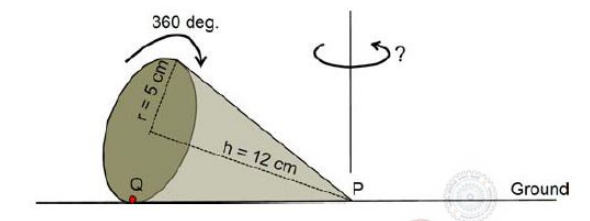
\includegraphics[width=0.5\textwidth]{figures/3.png}
\end{center}
By what angle (in radians) about P does the cone travel?}{3}
\begin{enumerate}
    \item[(A)] $\frac{5\pi}{12}$
    \item[(B)] $\frac{5\pi}{24}$  
    \item[(C)] $\frac{24\pi}{5}$
    \item[(D)] $\frac{10\pi}{13}$
\end{enumerate}

\vspace{0.5cm}

\questiona{In a company with 100 employees, 45 earn Rs. 20,000 per month, 25 earn Rs. 30,000, 20 earn Rs. 40,000, 8 earn Rs. 60,000, and 2 earn Rs. 150,000. The median of the salaries is}{4}
\begin{enumerate}
    \item[(A)] Rs. 20,000
    \item[(B)] Rs. 30,000  
    \item[(C)] Rs. 32,300
    \item[(D)] Rs. 40,000
\end{enumerate}

\vspace{0.5cm}

\questiona{P, Q, and R talk about S's car collection. P states that S has at least 3 cars. Q believes that S has less than 3 cars. R indicates that to his knowledge, S has at least one car. Only one of P, Q and R is right. The number of cars owned by S is}{5}
\begin{enumerate}
    \item[(A)] 0
    \item[(B)] 1  
    \item[(C)] 3
    \item[(D)] Cannot be determined
\end{enumerate}

\vspace{0.5 cm}

\questionb{"Here, throughout the early 1820s, Stuart continued to fight his losing battle to allow his sepoys to wear their caste-marks and their own choice of facial hair on parade, being again reprimanded by the commander-in-chief. His retort that 'A stronger instance than this of European prejudice with relation to this country has never come under my observations' had no effect on his superiors."

According to this paragraph, which of the statements below is most accurate?}{6}
\begin{enumerate}
    \item[(A)] Stuart's commander-in-chief was moved by this demonstration of his prejudice.
    \item[(B)] The Europeans were accommodating of the sepoys' desire to wear their caste-marks.  
    \item[(C)] Stuart's 'losing battle' refers to his inability to succeed in enabling sepoys to wear caste-marks.
    \item[(D)] The commander-in-chief was exempt from the European prejudice that dictated how the sepoys were to dress.
\end{enumerate}

\vspace{0.5cm}

\questionb{What is the sum of the missing digits in the subtraction problem below?

\[\begin{array}{c}
5\ \_\ \_\ \_\ \_\ \\ 
-4\ 8\ 8\ 9 \\ 
\hline 
1\ 1\ 1\ 1
\end{array}\]}{7}
\begin{enumerate}
    \item[(A)] 8
    \item[(B)] 10  
    \item[(C)] 11
    \item[(D)] Cannot be determined
\end{enumerate}

\vspace{0.5cm}

\questionb{Let $S_1$ be the plane figure consisting of the points $(x, y)$ given by the inequalities $|x - 1| \leq 2$ and $|y + 2| \leq 3$. Let $S_2$ be the plane figure given by the inequalities $x - y \geq -2$, $y \geq 1$, and $x \leq 3$. Let $S$ be the union of $S_1$ and $S_2$. The area of $S$ is}{8}
\begin{enumerate}
    \item[(A)] 26
    \item[(B)] 28  
    \item[(C)] 32
    \item[(D)] 34
\end{enumerate}

\vspace{0.5cm}

\questionb{Two very famous sportsmen Mark and Steve happened to be brothers, and played for country K. Mark teased James, an opponent from country E, "There is no way you are good enough to play for your country." James replied, "Maybe not, but at least I am the best player in my own family."

Which one of the following can be inferred from this conversation?}{9}
\begin{enumerate}
    \item[(A)] Mark was known to play better than James
    \item[(B)] Steve was known to play better than Mark  
    \item[(C)] James and Steve were good friends
    \item[(D)] James played better than Steve
\end{enumerate}

\vspace{0.5cm}

\questionb{The growth of bacteria (lactobacillus) in milk leads to curd formation. A minimum bacterial population density of 0.8 (in suitable units) is needed to form curd. In the graph below, the population density of lactobacillus in 1 litre of milk is plotted as a function of time, at two different temperatures, 25°C and 37°C.

\begin{center}
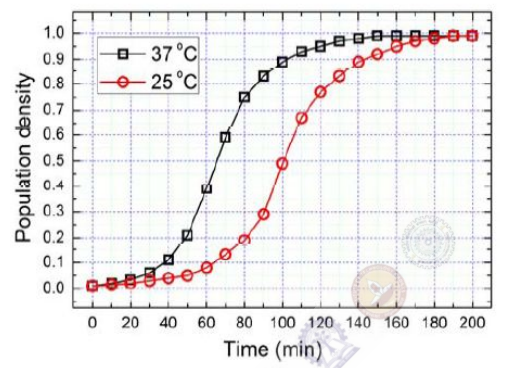
\includegraphics[width=0.5\textwidth]{figures/10.png}
\end{center}

Consider the following statements based on the data shown above:
\begin{enumerate}
\item[i.] The growth in bacterial population stops earlier at 37°C as compared to 25°C  
\item[ii.] The time taken for curd formation at 25°C is twice the time taken at 37°C
\end{enumerate}

Which one of the following options is correct?}{10}
\begin{enumerate}
    \item[(A)] Only i
    \item[(B)] Only ii  
    \item[(C)] Both i and ii
    \item[(D)] Neither i nor ii
\end{enumerate}

\vspace{0.5cm}

\vspace{0.5 cm}

% Technical Section
\section*{Technical Section}

\questiona{The Pritzker Architecture prize for the year 2016 has been awarded to}{1}
\begin{enumerate}
    \item[(A)] Alejandro Aravena
    \item[(B)] Frei Otto  
    \item[(C)] Stephen Breyer
    \item[(D)] Yung Ho Chang
\end{enumerate}

\vspace{0.5cm}

\questiona{As per the CPWD Handbook on Barrier Free and Accessibility, 2014, Government of India, the minimum length of a straight ramp in metre to raise a wheelchair to the plinth level of 600 mm, is \_\_\_\_\_.}{2}

\vspace{0.5cm}

\questiona{Tuscan and Composite orders are associated with}{3}
\begin{enumerate}
    \item[(A)] Greek Architecture
    \item[(B)] Islamic Architecture  
    \item[(C)] Byzantine Architecture
    \item[(D)] Roman Architecture
\end{enumerate}

\vspace{0.5cm}

\questiona{A pointed arch having two centres and radii greater than the span is known as}{4}
\begin{enumerate}
    \item[(A)] Lancet arch
    \item[(B)] Gothic arch  
    \item[(C)] Roman arch
    \item[(D)] Drop arch
\end{enumerate}

\vspace{0.5cm}

\questiona{The concepts of 'serial vision', 'punctuation' and 'closure' were proposed by}{5}
\begin{enumerate}
    \item[(A)] Le Corbusier
    \item[(B)] Louis Kahn  
    \item[(C)] Gordon Cullen
    \item[(D)] Kevin Lynch
\end{enumerate}

\vspace{0.5cm}

\questiona{In one litre of paint, volume of solid pigment and volume of non-volatile binder are 400 cc and 600 cc respectively. The Pigment Volume Concentration number of the paint is \_\_\_\_\_.}{6}

\vspace{0.5cm}

\questiona{'Cold joint' refers to the}{7}
\begin{enumerate}
    \item[(A)] expansion joint in large span concrete members
    \item[(B)] interface between an already setting concrete and a fresh batch of concrete  
    \item[(C)] structural crack arrested by embedding metal rods
    \item[(D)] joining of two similar metals in vacuum
\end{enumerate}

\vspace{0.5cm}

\questiona{Slenderness ratio of a column is represented as:}{8}
\begin{enumerate}
    \item[(A)] Effective length / Cross-sectional area
    \item[(B)] Effective length / Radius of gyration  
    \item[(C)] Actual length / Cross-sectional area
    \item[(D)] Actual length / Radius of gyration
\end{enumerate}

\vspace{0.5cm}

\questiona{Liquidated damage refers to the}{9}
\begin{enumerate}
    \item[(A)] cost borne by the contractor to rectify defects within defect-liability period
    \item[(B)] compensation paid on breach of contract to the affected party by the other party  
    \item[(C)] money paid by the insurance company to the owner of insured property if it is damaged
    \item[(D)] money earned by the owner from selling damaged property through auction
\end{enumerate}

\vspace{0.5cm}

\questiona{Which of the following processes is \textbf{NOT} used for corrosion resistance of cast iron?}{10}
\begin{enumerate}
    \item[(A)] Painting
    \item[(B)] Epoxy coating  
    \item[(C)] Quenching
    \item[(D)] Galvanizing
\end{enumerate}

\vspace{0.5cm}

\questiona{Data on 'households with one or more married couples sharing room with a person aged 12 years or more', is used for computing}{11}
\begin{enumerate}
    \item[(A)] housing density
    \item[(B)] housing shortage  
    \item[(C)] housing price
    \item[(D)] housing affordability
\end{enumerate}

\vspace{0.5cm}

\questiona{Excellence in Design for Greater Efficiency (EDGE) programme \textbf{DOES NOT} focus on}{12}
\begin{enumerate}
    \item[(A)] lower carbon emission  
    \item[(B)] greater resource efficiency  
    \item[(C)] cost effectiveness
    \item[(D)] labour safety
\end{enumerate}

\vspace{0.5cm}

\questiona{Select the right option representing strategic components arranged in ascending order of specified minimum area under Smart City Mission of Government of India.}{13}
\begin{enumerate}
    \item[(A)] Greenfield development - Redevelopment - Retrofitting
    \item[(B)] Redevelopment - Greenfield development - Retrofitting  
    \item[(C)] Retrofitting - Redevelopment - Greenfield development
    \item[(D)] Redevelopment - Retrofitting - Greenfield development
\end{enumerate}

\vspace{0.5cm}

\questiona{The grade-separated interchange suitable for 3-legged road intersection is:}{14}
\begin{enumerate}
    \item[(A)] Trumpet
    \item[(B)] Full Clover leaf  
    \item[(C)] Diamond
    \item[(D)] Partial Clover leaf
\end{enumerate}

\vspace{0.5cm}

\questiona{The design element provided to ensure safety of a vehicle travelling at a prescribed design speed along the curved segment of a highway is}{15}
\begin{enumerate}
    \item[(A)] shoulder
    \item[(B)] super-elevation  
    \item[(C)] median
    \item[(D)] footpath
\end{enumerate}

\vspace{0.5cm}

\questiona{Which of the following processes is \textbf{NOT} adopted in solid waste management?}{16}
\begin{enumerate}
    \item[(A)] Incineration
    \item[(B)] Pyrolysis  
    \item[(C)] Flocculation
    \item[(D)] Sanitary landfill
\end{enumerate}

\vspace{0.5cm}

\questiona{The principle of Eminent Domain is the power to}{17}
\begin{enumerate}
    \item[(A)] restrict exercise of rights in land through zoning and environmental laws
    \item[(B)] control land use  
    \item[(C)] retain land use
    \item[(D)] acquire and take possession of property in order to promote public interest
\end{enumerate}

\vspace{0.5cm}

\questiona{In which of the following models does the private partner own the revenue as well as the risk associated with the project for a limited period of time?}{18}
\begin{enumerate}
    \item[(A)] Build, Own, Operate (BOO)  
    \item[(B)] Build, Own, Operate, Transfer (BOOT)  
    \item[(C)] Design, Build, Finance, Operate (DBFO)
    \item[(D)] Design, Bid, Build (DBB)
\end{enumerate}

\vspace{0.5cm}

\questiona{In a multi-storied building, the type of plumbing system suitable for reusing the sullage for non-potable use is}{19}
\begin{enumerate}
    \item[(A)] single stack system
    \item[(B)] partially ventilated single stack system  
    \item[(C)] one pipe system
    \item[(D)] two pipe system
\end{enumerate}

\vspace{0.5cm}

\questiona{The unit for measuring sound absorption in a room is}{20}
\begin{enumerate}
    \item[(A)] Sabin
    \item[(B)] Phon  
    \item[(C)] Decibel
    \item[(D)] Hertz
\end{enumerate}

\vspace{0.5cm}

\questiona{In Geographic Information System, DEM represents information on}{21}
\begin{enumerate}
    \item[(A)] vegetation cover
    \item[(B)] soil type  
    \item[(C)] water table
    \item[(D)] topography
\end{enumerate}

\vspace{0.5cm}

\questiona{Minimum points required for GRIHA certification is}{22}
\begin{enumerate}
    \item[(A)] 35
    \item[(B)] 40  
    \item[(C)] 50
    \item[(D)] 60
\end{enumerate}

\vspace{0.5cm}

\questiona{ArchiCAD, Auto Desk Revit, Digital Project Designer (CATIA) and Vector Works Architect are examples of}{23}
\begin{enumerate}
    \item[(A)] Statistical Analysis software
    \item[(B)] GIS software  
    \item[(C)] BIM software
    \item[(D)] Image processing software
\end{enumerate}

\vspace{0.5cm}

\questiona{The CARTOSAT 2C satellite recently launched by ISRO}{24}
\begin{enumerate}
    \item[(A)] is a geo-synchronous satellite
    \item[(B)] is a part of IRNSS GPS satellite system  
    \item[(C)] was launched using a GSLV rocket
    \item[(D)] has high spatial resolution
\end{enumerate}

\vspace{0.5cm}

\questiona{Which of the following trees has a columnar form?}{25}
\begin{enumerate}
    \item[(A)] Delonix regia
    \item[(B)] Tamarindus indica  
    \item[(C)] Polyalthia longifolia
    \item[(D)] Callistemon lanceolatus
\end{enumerate}

\vspace{0.5cm}

\questionb{Match the architectural movements in \textbf{Group-I} with their proponents in \textbf{Group-II}.}{26}

\begin{tabularx}{\linewidth}{lXl}
\textbf{Group-I} & & \textbf{Group-II} \\
P. Deconstruction & & 1. Joseph Paxton \\
Q. Historicism & & 2. Kenzo Tange \\
R. Metabolism & & 3. Walter Gropius \\
S. Art Nouveau & & 4. Victor Horta \\
& & 5. Frank O. Gehry \\
\end{tabularx}

\begin{enumerate}
    \item[(A)] P-5, Q-1, R-2, S-4
    \item[(B)] P-5, Q-4, R-2, S-3  
    \item[(C)] P-5, Q-2, R-3, S-3
    \item[(D)] P-2, Q-4, R-1, S-5
\end{enumerate}

\vspace{0.5cm}

\questionb{Associate the historic buildings in \textbf{Group-I} with their predominant materials in \textbf{Group-II}.}{27}

\begin{tabularx}{\linewidth}{lXl}
\textbf{Group-I} & & \textbf{Group-II} \\
P. Lingaraj Temple, Bhubaneshwar, India & & 1. Red sandstone \\
Q. Victoria Memorial, Kolkata, India & & 2. Timber \\
R. Padmanabhapuram Palace, Thuckalay, India & & 3. Terracotta tiles \\
S. Humayun's Tomb, Delhi, India & & 4. Sandstone and laterite \\
& & 5. Marble \\
\end{tabularx}

\begin{enumerate}
    \item[(A)] P-1, Q-2, R-3, S-5
    \item[(B)] P-1, Q-4, R-3, S-5  
    \item[(C)] P-2, Q-1, R-3, S-4
    \item[(D)] P-4, Q-5, R-2, S-1
\end{enumerate}

\vspace{0.5cm}

\questionb{Match the terminologies in \textbf{Group-I} with their description in \textbf{Group-II}.}{28}

\begin{tabularx}{\linewidth}{lXl}
\textbf{Group-I} & & \textbf{Group-II} \\
P. Pruning & & 1. Cutting of trees \\
Q. Felling & & 2. Removing broken branches from trees for better growth \\
R. Hoeing & & 3. Maintaining moisture content in soil by a protective layer \\
S. Mulching & & 4. Indiscriminate cutting of branches to reduce the size of a tree \\
& & 5. Loosening the ground to remove weeds \\
\end{tabularx}

\begin{enumerate}
    \item[(A)] P-2, Q-1, R-5, S-3
    \item[(B)] P-2, Q-1, R-4, S-3  
    \item[(C)] P-2, Q-1, R-3, S-4
    \item[(D)] P-1, Q-2, R-3, S-1
\end{enumerate}

\vspace{0.5cm}

\questionb{A proposed housing will have HIG, MIG and LIG units on a site measuring 60,750 sq.m. The buildable area of each category of units with respect to the total buildable area will be 30\%, 50\% and 20\% respectively. The maximum allowable FAR is 2.5, ground coverage 45\% and height 15 m. The maximum buildable area in sq.m of HIG units, considering a floor height of 3 m for all categories will be \_\_\_\_\_.}{29}

\vspace{0.5cm}

\questionb{In 2011, the population of a town was 5,00,000 and the number of housing units were 1,00,000. Calculate the additional number of dwelling units (DU) required by 2031 so that there is no housing shortage. The assumptions are: 
\begin{itemize}
    \item[i.] 5\% decadal increase in population
    \item[ii.] New DU to be completed by 2021 is 10,000
    \item[iii.] Number of DU which will become non habitable by 2031 is 5,000
    \item[iv.] Average household size is 4.5
\end{itemize}}{30}

\vspace{0.5cm}

\questionb{Match the classical urban planning theories in \textbf{Group-I} with their proponents in \textbf{Group-II}.}{31}

\begin{tabularx}{\linewidth}{lXl}
\textbf{Group-I} & & \textbf{Group-II} \\
P. Concentric Zone Model & & 1. Berry and Horton \\
Q. Sector Model & & 2. Homer Hoyt \\
R. Multiple Nuclei Model & & 3. Ernest Burgess \\
S. Factorial Ecology & & 4. Shevky and Bell \\
& & 5. Harris and Ullman \\
\end{tabularx}

\begin{enumerate}
    \item[(A)] P-4, Q-1, R-3, S-5
    \item[(B)] P-3, Q-2, R-3, S-5  
    \item[(C)] P-2, Q-4, R-5, S-1
    \item[(D)] P-3, Q-2, R-5, S-1
\end{enumerate}

\vspace{0.5cm}

\questionb{Match the distinguished housing projects in \textbf{Group-I} with their architects in \textbf{Group-II}.}{32}

\begin{tabularx}{\linewidth}{lXl}
\textbf{Group-I} & & \textbf{Group-II} \\
P. Nagakin Capsule Tower, Tokyo, Japan & & 1. Walter Gropius \\
Q. Tara Apartment, New Delhi, India & & 2. Moshe Safdie \\
R. Habitat 67, Montreal, Canada & & 3. Ralph Erskine \\
S. Byker Wall, New Castle, England & & 4. Charles Correa \\
& & 5. Kisho Kurokawa \\
\end{tabularx}

\begin{enumerate}
    \item[(A)] P-5, Q-4, R-2, S-3
    \item[(B)] P-1, Q-3, R-4, S-5  
    \item[(C)] P-5, Q-2, R-1, S-4
    \item[(D)] P-5, Q-4, R-2, S-1
\end{enumerate}

\vspace{0.5cm}

\questionb{Match the development schemes by Government of India in \textbf{Group-I} with their objectives in \textbf{Group-II}.}{33}

\begin{tabularx}{\linewidth}{lXl}
\textbf{Group-I} & & \textbf{Group-II} \\
P. PMAY & & 1. Housing for All \\
Q. AMRUT & & 2. Rural cluster development \\
R. NRUM & & 3. Heritage city development \\
S. HRIDAY & & 4. Urban mobility improvement \\
& & 5. Urban rejuvenation \\
\end{tabularx}

\begin{enumerate}
    \item[(A)] P-1, Q-5, R-4, S-3
    \item[(B)] P-1, Q-5, R-2, S-3  
    \item[(C)] P-3, Q-5, R-1, S-2
    \item[(D)] P-4, Q-2, R-1, S-5
\end{enumerate}

\vspace{0.5cm}

\questionb{Match the international events in \textbf{Group-I} with their directives in \textbf{Group-II}.}{34}

\begin{tabularx}{\linewidth}{lXl}
\textbf{Group-I} & & \textbf{Group-II} \\
P. Earth Summit, Rio de Janeiro, 1992 & & 1. Kyoto Protocol \\
Q. UN Framework Convention on Climate Change, New York, 1992 & & 2. Agenda 21 \\
R. UN Sustainable Development Summit, New York, 2015 & & 3. Heritage conservation \\
S. Habitat II, Istanbul, 1996 & & 4. Agenda 2030 \\
& & 5. Housing for All \\
\end{tabularx}

\begin{enumerate}
    \item[(A)] P-1, Q-5, R-4, S-3
    \item[(B)] P-1, Q-5, R-2, S-3  
    \item[(C)] P-2, Q-1, R-4, S-5
    \item[(D)] P-2, Q-1, R-5, S-4
\end{enumerate}

\vspace{0.5cm}

\questionb{Match the planning techniques in \textbf{Group-I} with their salient features in \textbf{Group-II}.}{35}

\begin{tabularx}{\linewidth}{lXl}
\textbf{Group-I} & & \textbf{Group-II} \\
P. Land pooling & & 1. Assigning specific task on a short time horizon \\
Q. Action Plan & & 2. Assembling privately owned land parcels for development \\
R. Land sharing & & 3. Agreement for reallocation of land between occupiers and owners \\
S. Transfer of Development Rights & & 4. Assigning specific task on a long time horizon \\
& & 5. Incentive based voluntary shifting of FAR of a plot to another plot \\
\end{tabularx}

\begin{enumerate}
    \item[(A)] P-1, Q-5, R-4, S-3
    \item[(B)] P-2, Q-1, R-3, S-4  
    \item[(C)] P-2, Q-1, R-3, S-5
    \item[(D)] P-4, Q-2, R-1, S-5
\end{enumerate}

\vspace{0.5cm}

\questionb{For a symmetrical two dimensional truss as shown in the above figure, vertical force in kN acting on the member PQ is \_\_\_\_\_.}{36}

\begin{center}
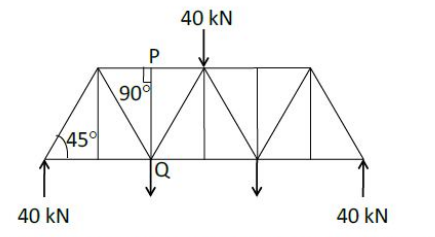
\includegraphics[width=0.5\textwidth]{figures/36.png}
\end{center}

\vspace{0.5cm}

\questionb{Value of bending moment in kN-m at point C for a beam as shown in the above figure is \_\_\_\_\_.}{37}

\begin{center}
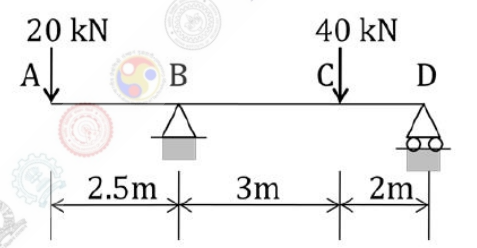
\includegraphics[width=0.5\textwidth]{figures/37.png}
\end{center}

\vspace{0.5cm}

\questionb{Fee of contractor for a project has the following provisions:
\begin{itemize}
    \item Basic fee = 15\% of actual cost of work incurred
    \item Bonus = 20\% of savings from estimated cost of work
    \item Penalty = 20\% of cost overrun
\end{itemize}
If the estimated cost of the project is Rs. 60,000, and the actual cost is Rs. 70,000, then the total fee of contractor in Rupees is \_\_\_\_\_.}{38}

\vspace{0.5cm}

\questionb{A site has a unidirectional slope of 30° with horizontal along its longer side. The projected dimensions of the site on the horizontal plane measures 30 m × 40 m. Using cut and fill method the site has to be levelled parallel to the horizontal plane. The minimum amount of earth to be excavated in cubic metre is \_\_\_\_\_.}{39}

\vspace{0.5cm}

\questionb{The optimistic, most-likely and pessimistic time for developing a new product are 12 months, 15 months and 17 months, respectively. Calculate the expected time in months.}{40}

\vspace{0.5cm}

\questionb{A circular plate inclined at an angle $\theta$ with horizontal plane generates an ellipse as top view with major axis and minor axis of 5 cm and 2.5 cm respectively. The value of $\theta$ in degrees is \_\_\_\_\_.}{41}

\vspace{0.5cm}

\questionb{Calculate the volume of cement in cubic metre required for making 10 cubic metre of M20 grade Plain Cement Concrete work, assuming the ratio of dry concrete mix to wet concrete mix as 1.52.}{42}

\vspace{0.5cm}

\questionb{One acre of agricultural land has been given on a lease till perpetuity at an annual rent of Rs. 10,000 to be paid at the end of each year. Net Present Value of the land parcel in Rupees assuming a discount rate of 5\% per annum is \_\_\_\_\_.}{43}

\vspace{0.5cm}

\questionb{In year 2001, a district with 4,000 manufacturing jobs had a 10\% share of total manufacturing jobs within the state. In year 2011, the state recorded 15\% drop in manufacturing jobs whereas, share of the district in total manufacturing jobs within the state increased to 15\%. Additional manufacturing jobs created in the district between year 2001 and 2011 is \_\_\_\_\_.}{44}

\vspace{0.5cm}

\questionb{Match the parameters in \textbf{Group I} with their units in \textbf{Group II}}{45}

\begin{tabularx}{\linewidth}{lXl}
\textbf{Group I} & & \textbf{Group II} \\
(P) Traffic flow & & 1. Metre \\
(Q) Traffic density & & 2. Cycles/second \\
(R) Right of Way & & 3. Seconds \\
(S) Traffic signal cycle length & & 4. Vehicle/km \\
& & 5. PCU/hr \\
\end{tabularx}

\begin{enumerate}
    \item[(A)] P-5, Q-4, R-1, S-2
    \item[(B)] P-5, Q-4, R-1, S-3  
    \item[(C)] P-5, Q-2, R-4, S-3
    \item[(D)] P-4, Q-5, R-1, S-3
\end{enumerate}

\vspace{0.5cm}

\questionb{Match the planning tasks in \textbf{Group I} with the tools of analysis in \textbf{Group II}.}{46}

\begin{tabularx}{\linewidth}{lXl}
\textbf{Group I} & & \textbf{Group II} \\
(P) Population projection & & 1. Input-Output Analysis \\
(Q) Regional resource allocation & & 2. Hardy Cross Method \\
(R) Trip distribution & & 3. Cohort Analysis \\
(S) Design of water distribution network & & 4. Gravity Model \\
& & 5. Moving observer method \\
\end{tabularx}

\begin{enumerate}
    \item[(A)] P-3, Q-1, R-4, S-2
    \item[(B)] P-3, Q-5, R-4, S-1  
    \item[(C)] P-5, Q-1, R-3, S-4
    \item[(D)] P-1, Q-3, R-5, S-2
\end{enumerate}

\vspace{0.5cm}

\questionb{Match the land use classes in \textbf{Group I} with the use zones in \textbf{Group II}.}{47}

\begin{tabularx}{\linewidth}{lXl}
\textbf{Group I} & & \textbf{Group II} \\
(P) Transportation & & 1. Sports complex \\
(Q) Commercial & & 2. Heritage and conservation areas \\
(R) Public and Semi-public & & 3. Burial ground \\
(S) Recreational & & 4. BRT corridor \\
& & 5. Service sector \\
\end{tabularx}

\begin{enumerate}
    \item[(A)] P-4, Q-1, R-3, S-5
    \item[(B)] P-5, Q-3, R-1, S-2  
    \item[(C)] P-4, Q-5, R-1, S-2
    \item[(D)] P-4, Q-5, R-3, S-1
\end{enumerate}

\vspace{0.5cm}

\questionb{Associate the structural systems in \textbf{Group I} with the buildings in \textbf{Group II}.}{48}

\begin{tabularx}{\linewidth}{lXl}
\textbf{Group I} & & \textbf{Group II} \\
(P) Folded plates & & 1. Kurilpa Bridge, Brisbane \\
(Q) Shell & & 2. Eden Project, Cornwall \\
(R) Tensegrity & & 3. Riverside Museum, Glasgow \\
(S) Pneumatic & & 4. MIT Auditorium, Boston \\
& & 5. 30, St. Mary Axe, London \\
\end{tabularx}

\begin{enumerate}
    \item[(A)] P-3, Q-4, R-1, S-2
    \item[(B)] P-5, Q-4, R-3, S-1  
    \item[(C)] P-3, Q-2, R-1, S-5
    \item[(D)] P-1, Q-3, R-4, S-2
\end{enumerate}

\vspace{0.5cm}

\questionb{As per National Building Code of India, 2005, the maximum number of occupants per unit exit width of a doorway is 60, where unit exit width is 500 mm. The maximum permissible occupants in a theatre having four number of 2.2 m wide doors will be \_\_\_\_\_.}{49}

\vspace{0.5cm}

\questionb{Match the instruments in \textbf{Group I} with the corresponding tests in \textbf{Group II}.}{50}

\begin{tabularx}{\linewidth}{lXl}
\textbf{Group I} & & \textbf{Group II} \\
(P) Pycnometer & & 1. Initial and final setting time \\
(Q) Brinell's Apparatus & & 2. Abrasion test \\
(R) Los Angeles Apparatus & & 3. Surface hardness test \\
(S) Vicat's Apparatus & & 4. Slump test \\
& & 5. Apparent Specific gravity \\
\end{tabularx}

\begin{enumerate}
    \item[(A)] P-5, Q-3, R-2, S-1
    \item[(B)] P-5, Q-4, R-2, S-1  
    \item[(C)] P-3, Q-2, R-1, S-5
    \item[(D)] P-2, Q-3, R-4, S-1
\end{enumerate}

\vspace{0.5cm}

\questionb{Water flows through a constricted circular pipe whose diameter at the constricted end is half of the non-constricted end. Velocity of water at the non-constricted end is 2 m/s. Velocity of water in m/s at the constricted end using the principle of continuity of flow is \_\_\_\_\_.}{51}

\vspace{0.5cm}

\questionb{A drainage basin of 180 hectares comprises 40\% wooded area, 45\% grassed area and 15\% paved area. Runoff coefficients for wooded, grassed and paved areas are 0.01, 0.2 and 0.95 respectively. The composite runoff coefficient for the drainage basin is \_\_\_\_\_.}{52}

\vspace{0.5cm}

\questionb{A fluorescent light source consumes 40 W electric power and has a luminous efficacy of 40 lm/W. Illumination in lux at a distance of 3 m from this light source is \_\_\_\_\_.}{53}

\vspace{0.5cm}

\questionb{A room measures 3 m (width) × 4 m (length) × 3 m (height). The outdoor temperature is 36°C. The volumetric specific heat of air is 1300 J/m$^3$°C. The ventilation heat flow rate in Watts required to attain an internal room temperature of 26°C with 3 air changes per hour is \_\_\_\_\_.}{54}

\vspace{0.5cm}

\questionb{Match the equipment in \textbf{Group-I} with their applications in \textbf{Group-II}.}{55}

\begin{tabularx}{\linewidth}{lXl}
\textbf{Group-I} & & \textbf{Group-II} \\
P. PIR & & 1. Air conditioning \\
Q. FCU & & 2. Lighting \\
R. OLED & & 3. Power generation \\
S. BIPV & & 4. Motion detection \\
& & 5. Daylight sensing \\
\end{tabularx}

\begin{enumerate}
    \item[(A)] P-4, Q-5, R-2, S-1
    \item[(B)] P-1, Q-4, R-5, S-3  
    \item[(C)] P-4, Q-1, R-2, S-3
    \item[(D)] P-4, Q-2, R-5, S-1
\end{enumerate}

\vspace{0.5cm}

\vspace{5cm}
\begin{center}
\textbf{END OF THE QUESTION PAPER}
\rule{\textwidth}{0.5pt} 
\end{center}

\end{document}
